\lstset{basicstyle=\small\ttfamily,
        emphstyle=\bfseries,
        columns=fixed,
        numbers=left,xleftmargin=2em,frame=single,framexleftmargin=1.5em,
        moredelim=*[l][\textit]{//},
        moredelim=*[l][\bfseries]{\#},
        literate={...}{\dots}3
} 

Parallel programming models ~\cite{Blumofe:PPoPP1995, Reinders2007, Bauer2012, OmpSs},  are widely used to facilitate the programming of parallel codes for multi-core systems.
These programming models offer an abstraction layer to the programer so that multi-threaded programming of an application becomes easier.
They support code annotations that the programmer can add to the application's sequential code and transform it into parallel.
These annotations include the specification of parallel loops, atomic operations, critical regions or task clauses.

Our main focus in this thesis is the task annotation with dependency tracking which OpenMP~\cite{OpenMP} supports since its 4.0 release~\cite{OpenMP4.0:Manual2015}.
A task is a piece of code{\footnote{A piece of code can be a function or a code block.} in the application that can execute simultaneously to other tasks and cooperatively produce results.
In a parallel application there can be many tasks that perform the same computations on different data or tasks that perform different computations on the same data.
By using task annotations, the programmer decomposes the application into tasks and specifies the input and output data dependencies between them.
Parallel programming models typically consist of two parts; a compiler and a runtime system.
The compiler is responsible to parse the code annotations and translate them to code by adding calls to the programming model's runtime system.
The runtime system consists of software threads and is responsible for the efficient execution of the tasks with respect to the data dependencies as well as the availability of resources.
This thesis mainly focuses on enhancements of the runtime system in parallel programming models.

The runtime system creates and manages the software threads for the execution of the tasks. 
Typically one software thread is being bound to each core. 
One of the threads is the \textit{master thread}, and the rest are the \textit{worker threads}. 
The master thread starts executing the compiler generated application's code sequentially and creates the tasks as it encounters them. 
Following task creation, is the analysis of the dependencies of the created task and the insertion of it in the Task Dependency Graph (TDG).

A TDG is a distributed graph structure that connects each task of the application with the rest of the tasks according to their existing input and output data dependencies.
A dependency tracking mechanism is responsible for the maintenance of the input and output data of a task.
Within this mechanism, the runtime system tracks the memory addresses that tasks write or read and according to this, it manages the tasks that are ready for execution\footnote{When the input data of a task is produced, the task can start execution.}.
Tasks that their input data have been produced are marked as \textit{ready} and can start execution, while tasks that are still waiting for input are postponed until their inputs are produced by other executing tasks.

To enable the efficient parallel execution of the tasks, the scheduler of the runtime system keeps track of the available tasks to be executed and manages the task-to-thread allocation.
To do this, the scheduler maintains a \textit{ready queue} and when all of a tasks dependencies are satisfied (i.e., the task becomes \textit{ready}) it is inserted in the \textit{ready queue}. 
All threads have access to this queue which is a first-in-first-out data structure; whenever a thread becomes idle, it pops the next task from the queue and executes it. 
In this thesis we make use of OmpSs~\cite{OmpSs}, a mainstream task-based programming model and the main influence of the updated OpenMP~4.0~\cite{OpenMP}.

\subsection{OmpSs Programming Model}
\kc{Transform it to OpenMP??}
The OmpSs programming model is a task-based programming model that offers a high level abstraction to the implementation of parallel applications for various homogeneous and heterogeneous architectures~\cite{OmpSs_PPL11,OmpSs}. 
As a task-based programming model, OmpSs enables the annotation of function declarations with the task directive, which declares a task. 
Every invocation of a such function creates a task that is executed concurrently with other tasks or parallel loops. 
OmpSs also supports task dependencies and it uses the StarSs~\cite{StarSs} dependency tracking mechanisms. 
OmpSs is built with the support of the Mercurium compiler, responsible for the translation of the OmpSs annotation clauses to source code, and the Nanos++ runtime system~\cite{nanos}, responsible for the internal creation and execution of the tasks.

As a task-based parallel programming model, OmpSs enables the annotation of function declarations with the task directive. 
If a function is declared as a task, then every invocation of this function creates a task that is executed concurrently with other tasks or parallel loops. 
The accessible data to each task are the arguments of the function. 
OmpSs uses the StarSs~\cite{StarSs} dependency tracking mechanisms and each task may be annotated with the \textit{in}, \textit{out}, \textit{inout} clauses. 
These clauses allow the specification of scalars, arrays and pointers as input, output or input and output data of a task. 
The implementation of a barrier is supported under the \textit{taskwait} clause, and it can also be used with the addition of the \textit{on} clause, to declare a barrier for the group of tasks that produce a specific piece of data. 
These original OmpSs features can now be found in OpenMP 4.0~\cite{OpenMP}.

Nanos++ is an environment designed to serve as the runtime platform of OmpSs. 
It provides device support for heterogeneity and includes different plug-ins for implementations of scheduling policies, throttling policies, thread barriers, dependency tracking mechanisms, work-sharing and instrumentation. 
This design allows to maintain the runtime features by adding or removing plug-ins. 
Thus, the implementation of a new scheduler, or the support of a new architecture becomes simple.

The implementations of the different scheduling policies in Nanos++ perform various actions on the states of the tasks. 
A task is \textit{created} if a call to this task is discovered but it is waiting until all its inputs are produced by other previous tasks. 
When all the input dependencies are satisfied, the task becomes \textit{ready}. 
The ready tasks of the application at a given point in time are inserted in the \textit{ready queues} as stated by the scheduling policy. 
Ready queues can be thread-private or shared among multiple threads. 
When a thread becomes idle, the scheduling policy picks a task from the ready queues for that thread to execute. 

The Nanos++ internal data structures support task prioritization. 
The task priority is an integer field inside the task descriptor that rates the importance of the task. 
If the scheduling policy supports priorities, the ready queues are implemented as \textit{priority queues}. 
In a priority queue, tasks are sorted in a decreasing order of their priority. 
The insertion in a priority queue is always ordered and the removal of a task is always from the head of the queue, i.e., the task with the highest priority. 
The priority of a task can be either set in user code, by using the \textit{priority} clause, which accepts an integer priority value or expression, or dynamically  by the scheduling policy, as is described in the next section.



%%%%% This should be in the TaskGenX Chapter background. It is more specific to this implementation %%%%%%%

%\texttt{Memalloc} is performing the memory allocation for the task and its arguments.
%Next is a runtime call, which is the \texttt{createTask}, responsible for the linking of the task with the runtime system.
%At this point a task is considered \textit{created} and below are the three possible states of a task inside the runtime system:
%\begin{itemize}
%\item \textit{Created:} A task is initialized with the appropriate data and function pointers and it is inserted in the Task Dependency Graph (TDG). The insertion of a task in the TDG implies that the data dependencies of the tasks have been identified and the appropriate data structures have been created and initialized. 
%\item \textit{Ready:} When all the data dependencies of a created task have been satisfied, the task is ready and it is inserted in the \textit{ready queue} where it waits for execution. 
%\item \textit{Finished:} When a task has finished execution and has not been deleted yet.
%\end{itemize}

%Listing~\ref{taskCreation} shows the pseudo-code for the task creation step within the runtime.
%The \texttt{createTask} function is first initializing the task by copying the corresponding data to the allocated memory as well as connecting the task to its parent task (\texttt{initAndSetupTask}).
%After this step, the task is ready to be inserted in the TDG. 
%The TDG is a distributed and dynamic graph structure that the runtime uses to keep the information about the current tasks of the application. 
%The insertion of a task in the TDG is done by the \texttt{insertToTDG} function.
%This function takes as arguments a list with all the memory addresses that are to be written or read by the task (\texttt{dList}), and the task itself.
%Listing~\ref{insertTDG} shows the pseudo-code for the TDG insertion. 
%If for a task the \texttt{dList} is empty (line 2), this means that there are no memory addresses that need to be tracked during the execution; thus, the task is marked as \textit{ready} by pushing it to the \textit{ready queue} (line 3).
%Each entry of \texttt{dList} contains the actual memory address as well as the access type (read, write or read-write).
%The runtime keeps a distributed unified dependency tracking structure, the \texttt{depMap} where it stores all the tracked memory addresses together with their writer and reader tasks.
%For each item in the \texttt{dList} the runtime checks if there is an existing representation inside the \texttt{depMap} (line 8).
%If the memory address of an entry of the \texttt{dList} is not represented in the \texttt{depMap}, it is being added as shown in line 9.
%If the address of a \texttt{dList} item exists in the \texttt{depMap}, this means that a prior task has already referred to this memory location, exhibiting a data dependency.
%According to the access type of \texttt{d}, the readers and the writers of the specific address are updated in the \texttt{depMap} (lines 10-15).
%
%To reduce the lookup into the \texttt{depMap} calls, every time the contents of a memory address are modified, the tasks keep track of their \textit{successors} as well as the number of \textit{predecessors}.
%The \textit{successors} of a task are all the tasks with inputs depending on the output of the current task.
%The \textit{predecessors} of a task are the tasks whose output is used as input for the current task.
%When a \texttt{read} access is identified, the task that is being created is added to the list of successors of the last writer task, as shown on line 20 of Listing~\ref{taskCreation}.
%
%As tasks are executed, the dependencies between them and their successors are satisfied. 
%So the successor tasks that are waiting for input, eventually become \textit{ready} and are inserted to the ready queue.
%When a task goes to the \textit{finished} state, the runtime has to perform some actions in order to prepare the successor tasks for execution.
%These actions are described in Listing~\ref{taskFinish}.
%The runtime first updates the \texttt{depMap} to remove the possible references of the task as reader or writer (line 2).
%Then, if the task does not have any successors, it can safely be deleted (line 3).
%If the task has successors, the runtime traverses the successor list and for each successor task it decreases its predecessor counter (lines 5-6).
%If for a successor task its predecessor counter reaches zero, then this task becomes \textit{ready} and it is inserted in the \textit{ready queue} (lines 7-8).
%\begin{lstlisting}[float, emph={is, void,if,return,Dependency,DepList,Data,Task,not,for,true,and,break}, captionpos=b, caption={Pseudo-code for TDG insertion},label=insertTDG, emph={[2]mat}, emphstyle={[2]}, aboveskip={0\baselineskip}, frame=tb, belowskip={0\baselineskip}]
%void insertToTDG(DepList dList, Task t) {
% if( dList is empty ) {
%   readyQ->push(t);
%   return;
% }
% Dependency entry;
% for( d in dList ) {
%   entry = depMap[d.address()];
%   if(entry==NULL) depMap.add(entry, t);
%   if(d.accessType() == "write")
%     entry.addLastWriter(t);
%   if(d.accessType() == "read") {
%     entry.addReader(t);
%     entry.lastWriter()->addSuccessor(t);
%   }
% }
%}
%\end{lstlisting}
%The runtime activity takes place at the task state changes. 
%One state change corresponds to the task creation, so a task from being just allocated it becomes \textit{created}. 
%At this point the runtime prepares all the appropriate task and dependency tracking data structures as well as inserts the task into the TDG.
%The second change occurs when a task from being \textit{created} it becomes \textit{ready};
%this implies that the input dependencies of this task are satisfied so the runtime schedules and inserts the task into the ready queue.
%The third change occurs when a running task finishes execution. 
%In this case, following our task states, the task from being \textit{ready} it becomes \textit{finished}; this is followed by the runtime updating the dependency tracking data structures and scheduling possible successor tasks that become ready. 
%For the rest of the paper we will refer to the first state change runtime activity as the task creation overheads (\textit{Create}).
%For the runtime activity that takes place for the following two state changes (and includes scheduling and dependence analysis) we will use the term runtime overheads (\textit{Runtime}).

%\subsection{Motivation}
%
%\begin{figure}[t!]%
%	\centering
%	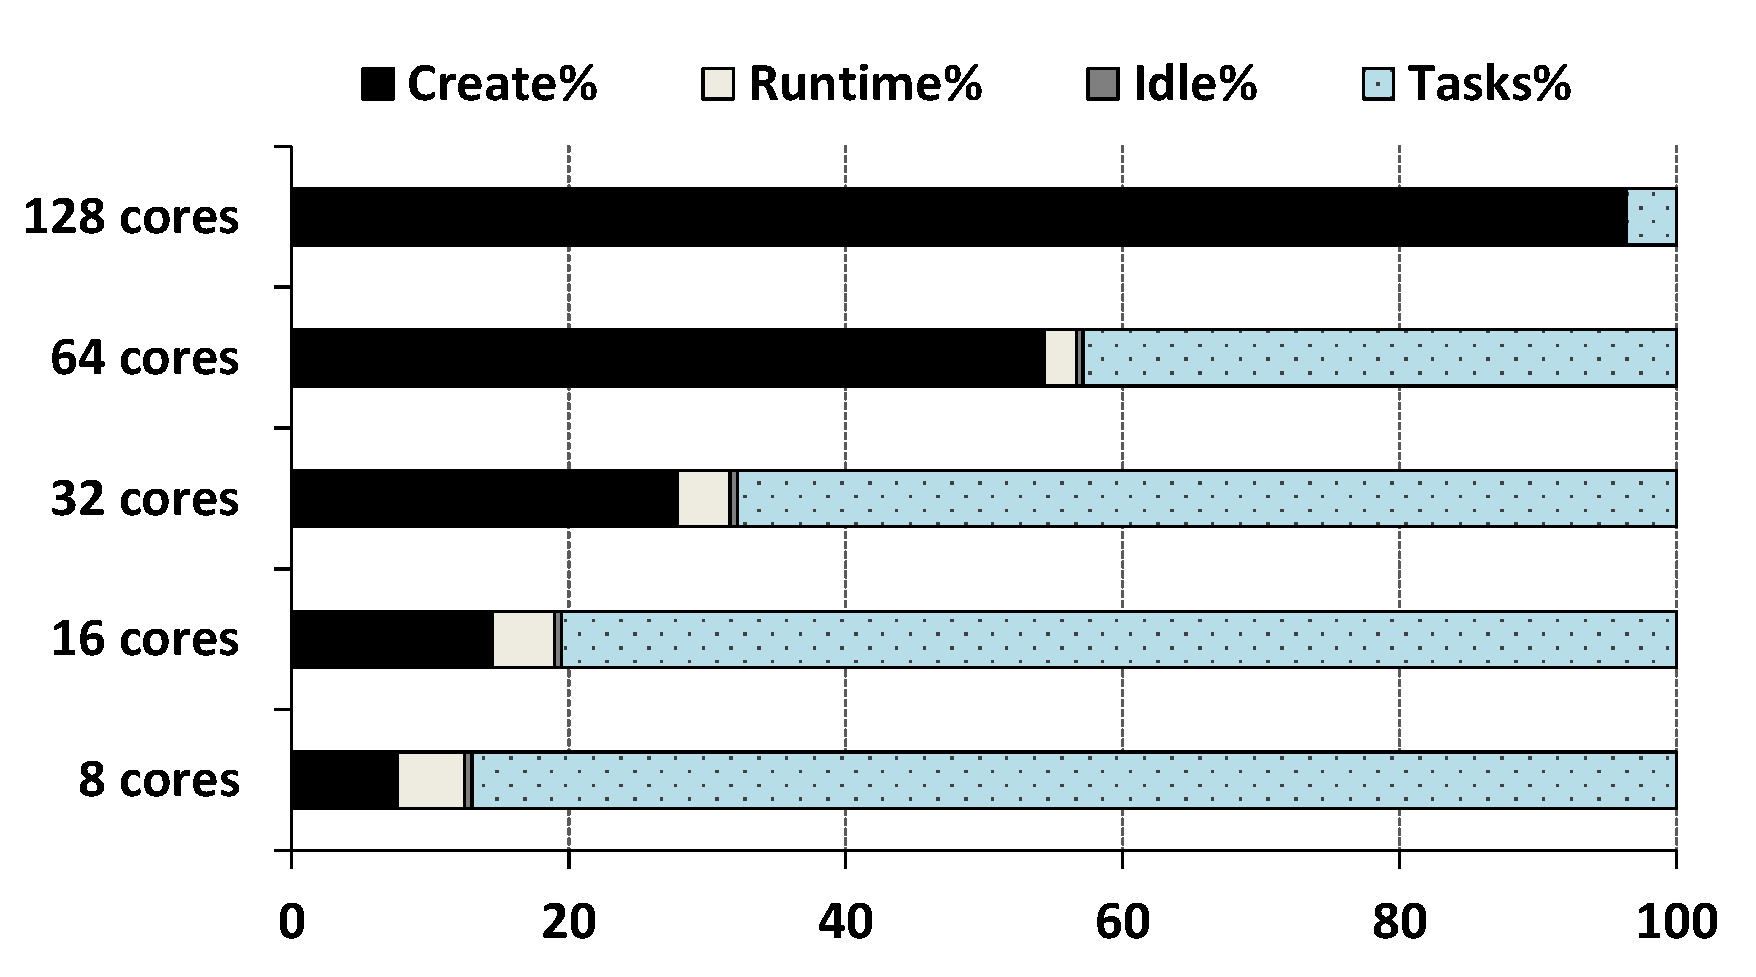
\includegraphics[width=0.75\columnwidth]{figures/master_thread.pdf}
%	\caption{Master thread activity for Cholesky as we increase the number of cores.}
%	%\caption{Performance improvements on a big.LITTLE processor with different $(F,N)$ configurations, where $F$ is the total number of big cores and $N$ the total number of cores. Results are normalized to running on four little cores with pinned Pthreads.}%
%	\label{fig:master_thread}%
%\end{figure}
%
%Figure~\ref{fig:master_thread} shows the runtime activity of the master thread during the execution of the Cholesky{\footnote{Details about the benchmarks used are in Section~\ref{sec:experimental}} benchmark on 8, 16, 32, 64 and 128 cores\footnote{The experimental set-up is explained in Section~\ref{sec:experimental}}.
%The execution time represented here is the wall clock time during the parallel region of the benchmark.
%Each one of the series represents a different runtime overhead from the ones described above.
%%\textit{Create} represents the \textit{Creation} step, 
%%\textit{Runtime} refers to the \textit{Finish} step, \textit{Idle} shows the master thread's idle time and the \textit{Tasks} is the time spent on task execution. 
%The percentage of time spent on task creation is increasing as we increase the number of cores.
%This is because the creation overhead is invariant of core count: the more we reduce the application's execution time by adding resources the more important this step becomes in terms of execution time.
%In contrast, the task execution time percentage is decreased as we increase the number of cores because the computational activity is being shared among more resources.
%One way to reduce the task creation overhead is by introducing nested parallelism. 
%In this programming technique, every worker thread is able to generate tasks thus the task creation is spread among cores and its overhead is reduced.
%However, not all applications can be implemented with this parallelization technique and there are very few applications using this scheme.
%\textit{Runtime} decreases as we increase the number of cores because this activity is also shared among the resources.
%This is because this part of the runtime takes place once the tasks finish execution and new tasks are being scheduled. 
%So the more the resources, the less the runtime activity per thread, therefore less activity for the master thread.
%%\kc{explain that this is wall clock time. The \textit{Runtime} activity is actually the part of the master thread but also the worker threads are performing this activity while the Create is only within the master thread.}
%
%\begin{lstlisting}[float, emph={void,if,return,Task,for,not,true,and,break}, captionpos=b, caption={Pseudo-code for task$\_$finish runtime activity.},label=taskFinish, emph={[2]mat}, emphstyle={[5]}, aboveskip={0\baselineskip}, frame=tb, belowskip={0\baselineskip}]
%void task_finish(Task *t) {
%  depMap.removeReaderWriter(t);
%  if(t->successors.empty()) delete t;
%  else {
%    for( succ in t->successors ) {
%      succ.decreasePredecessors();
%      if(succ.numPredecessors == 0) 
%        readyQ->push(succ);
%    }
%  }
%}
%\end{lstlisting}
%
%Our motivation for this work is the bottleneck introduced by task creation as shown in Figure~\ref{fig:master_thread}.
%Our runtime proposal decouples this piece of the runtime and accelerates it on a specialized hardware resulting in higher performance.
%
